\documentclass{beamer}
\usepackage{../../shared/styles/custom}
\usepackage{../../shared/styles/conventions}

\graphicspath{ {../assets/subgradient/figures/} }


\title{Subgradient}
\date{\today}
\author{Nipun Batra}
\institute{IIT Gandhinagar}
\begin{document}
  \maketitle
  
  
  
% \section{Linear Regression}

\begin{frame}{Subgradient }
\begin{itemize}
	
	
	\item Generalises gradient to convex but non-differentiable problems
	\item Examples:
	\begin{itemize}
		\item $f(x) = |x|$
	\end{itemize}
	
\end{itemize}
\end{frame}

\begin{frame}{Task at hand}
\begin{itemize}

\item TASK: find derivative of $f(x)$ at $x = x_0$
\end{itemize}
\begin{figure}
    \centering
    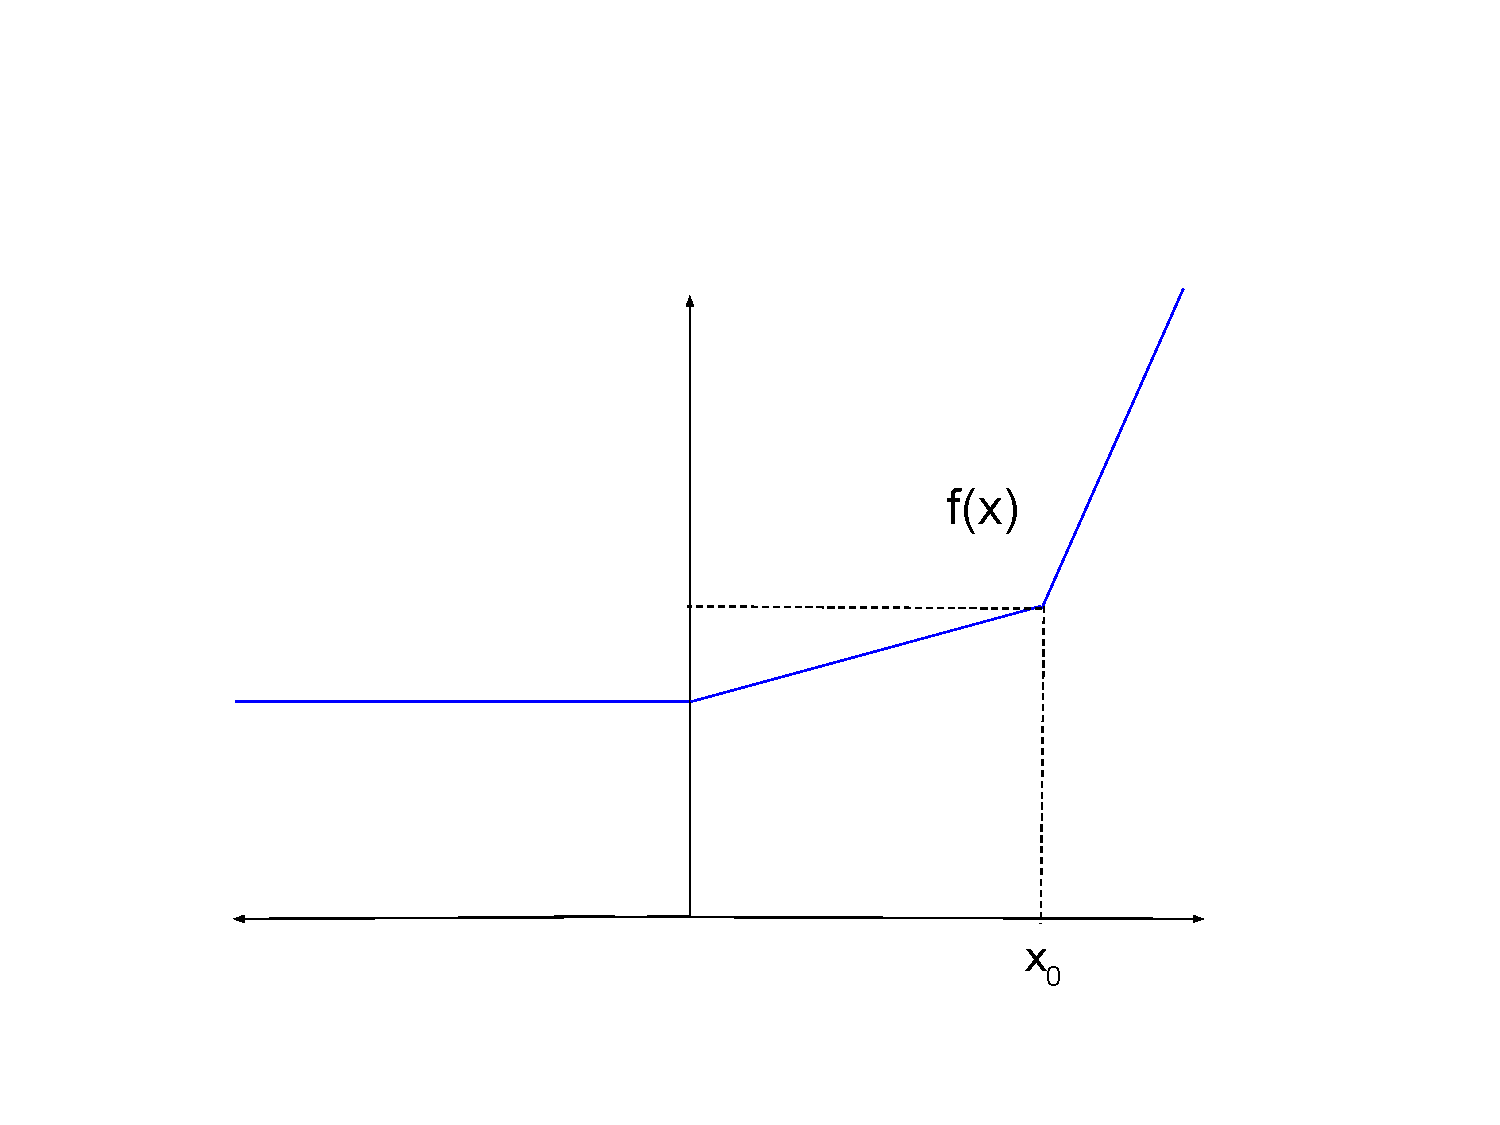
\includegraphics[scale = 0.25]{subgradient_1.pdf}
    
    \label{fig:Non-differentiable function}
\end{figure}
	

\end{frame}

\begin{frame}{Solution}

\begin{itemize}
\item Construct a differentiable $g(x)$ 
\begin{itemize}
    \item Intersecting $f(x)$ at $x = x_0$
    \item Below or on $f(x)$ for all x
\end{itemize}
\end{itemize}
\begin{figure}
    \centering
    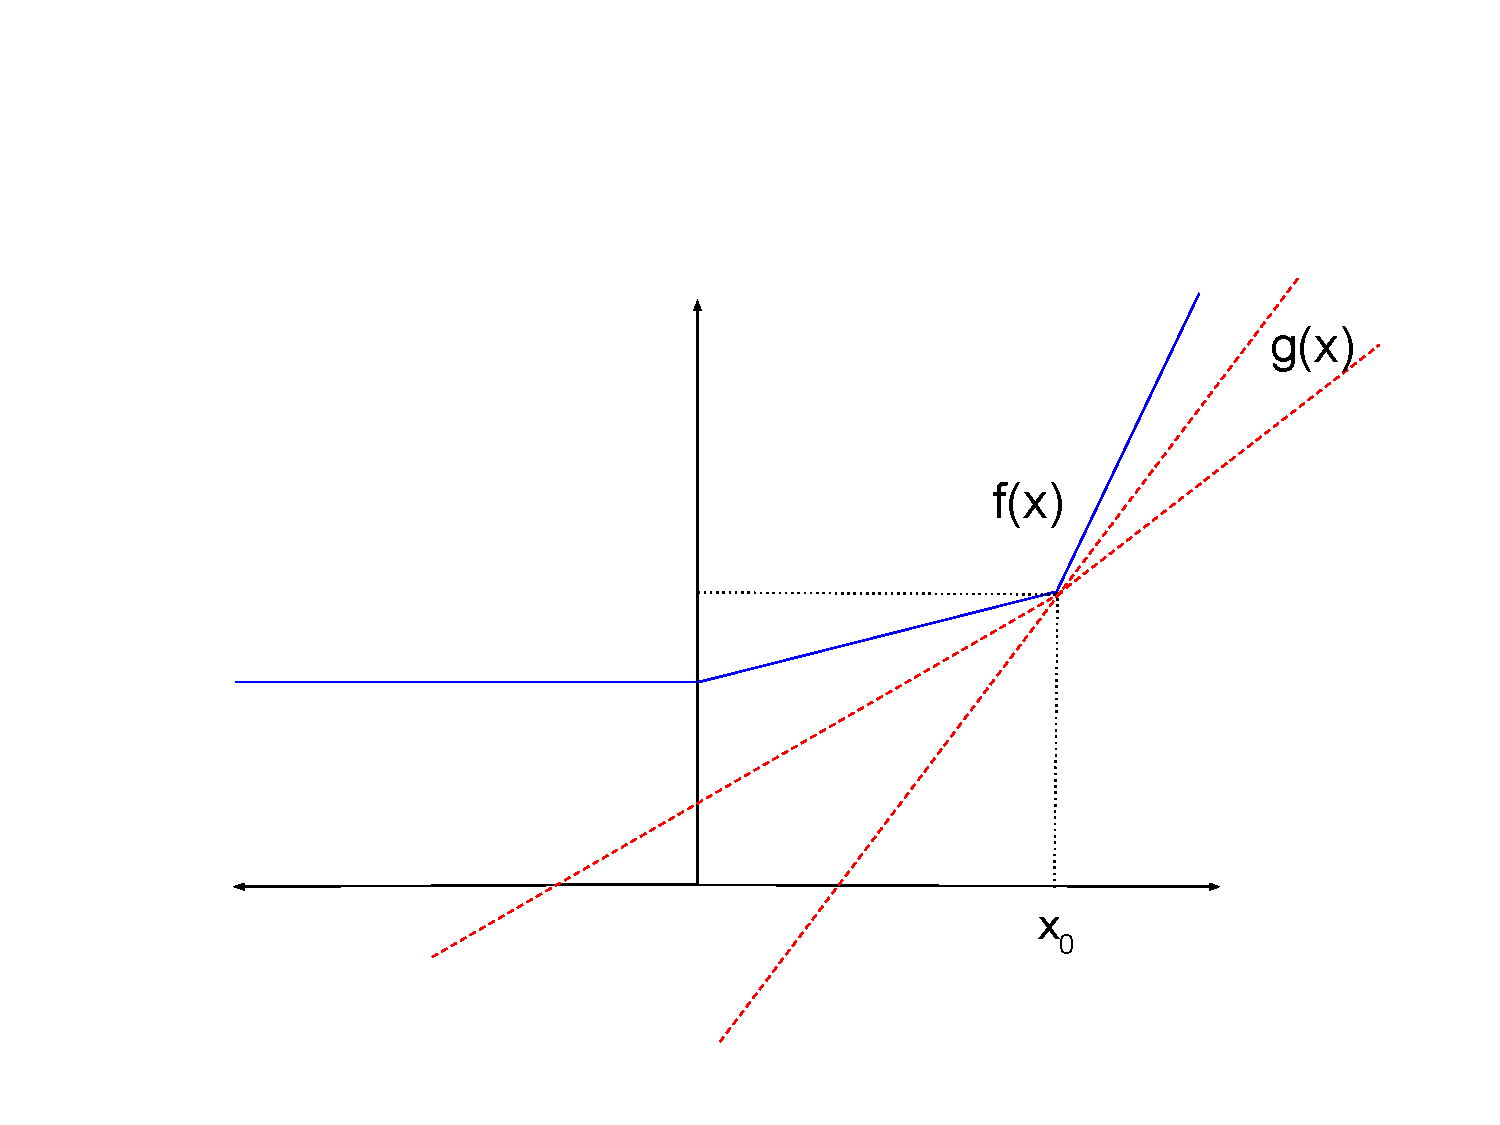
\includegraphics[scale = 0.25]{subgradient_2.pdf}
    \label{fig:my_label}
\end{figure}
\end{frame}

\begin{frame}{Solution}

\begin{itemize}
\item Compute slope of $g(x)$ at $x = x_0$
\end{itemize}
\begin{figure}
    \centering
    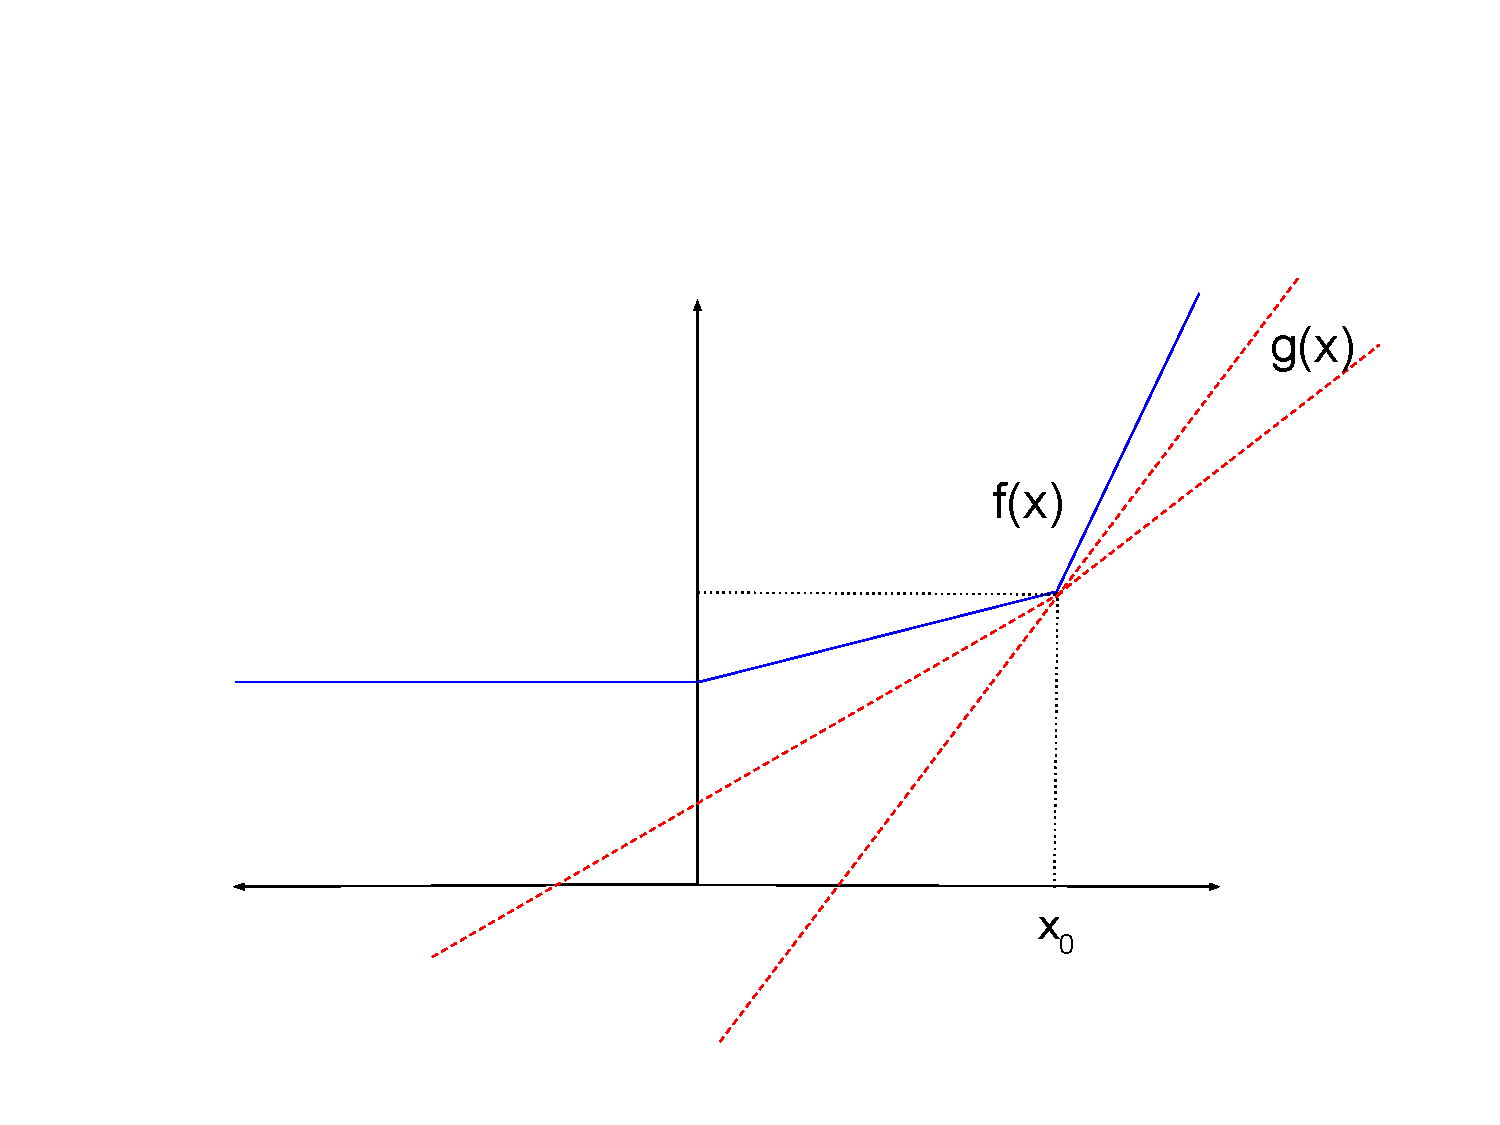
\includegraphics[scale = 0.25]{subgradient_2.pdf}
    
    \label{fig:my_label}
\end{figure}
\end{frame}

\begin{frame}{Another Example: $f(x) = |x|$}

\begin{itemize}
\item Subgradient of $f(x)$ belongs to $[-1, 1]$
\end{itemize}
\begin{figure}
    \centering
    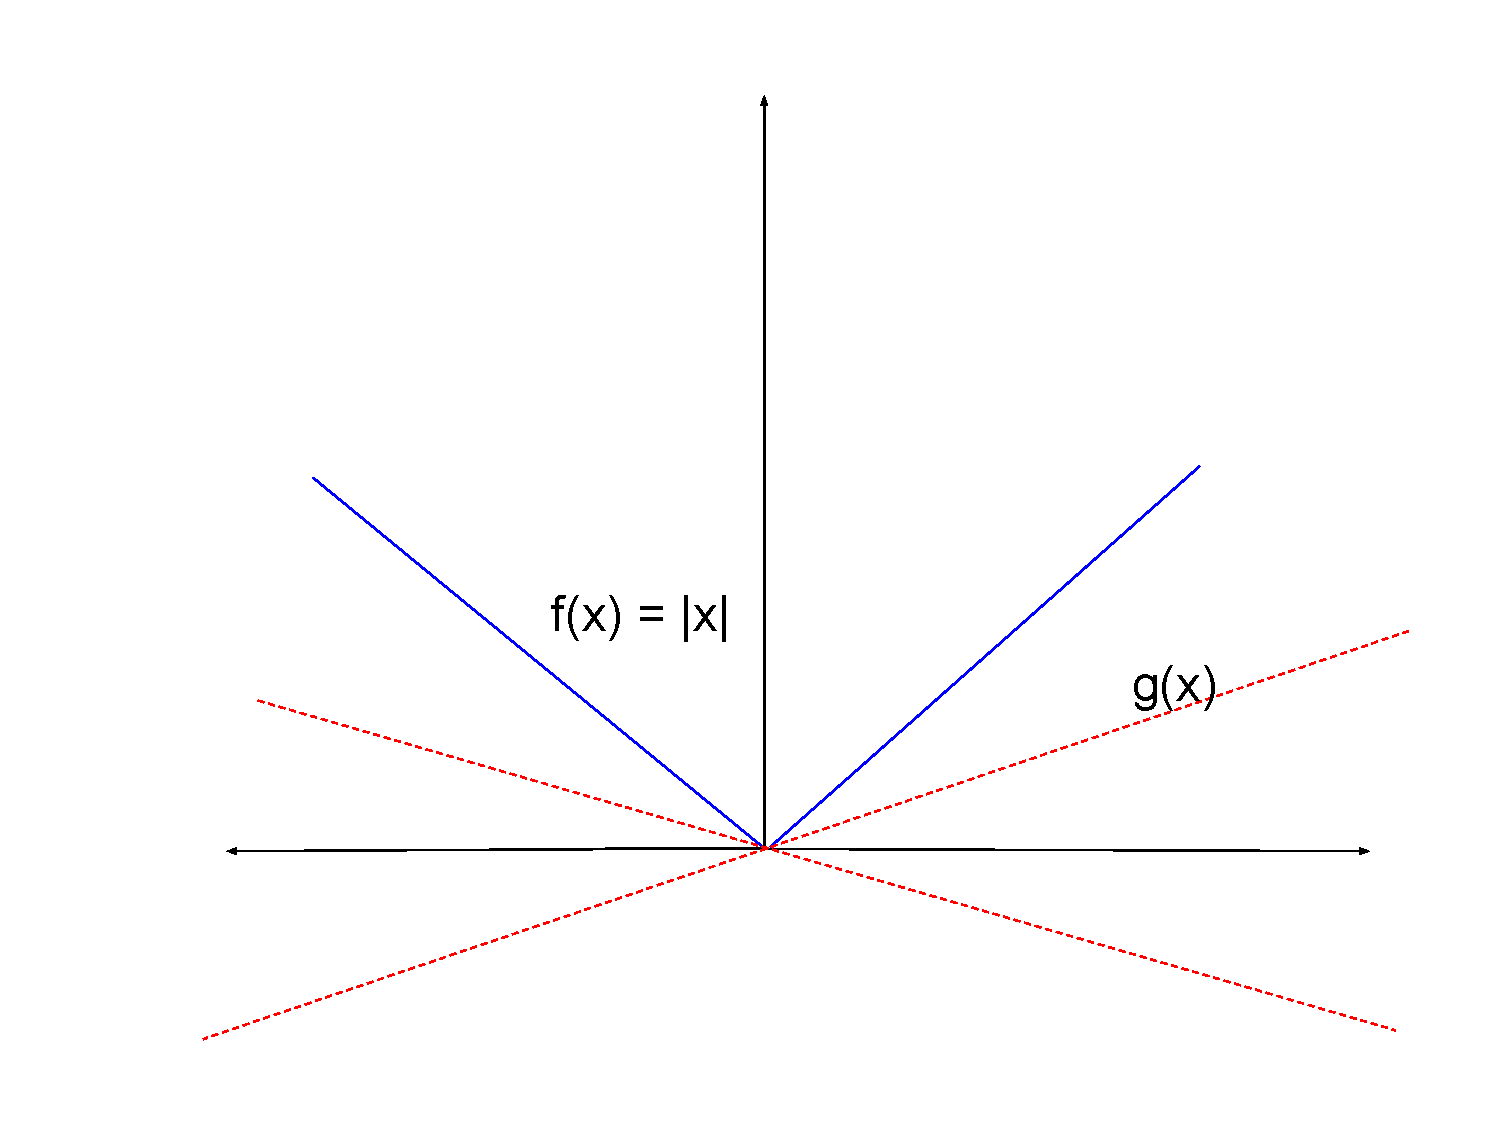
\includegraphics[scale = 0.25]{subgradient_3.pdf}
    \label{fig:my_label}
\end{figure}
\end{frame}




\end{document}
